\section{Introduction}

\textbf{Domain and motivation.} A cone penetration test (CPT) pushes a cone into the ground and records the
cone resistance \qc{} (MPa) with depth. High \qc{} means stiff ground; low-\qc{} layers indicate soft material
that matters for design. Each test samples one vertical line, so the ground between tests must be inferred.
Investigations usually fix the number and positions of CPTs in advance and complete them all, although
some add little information. Fewer tests save money, and finishing earlier can bring a whole project forward.

\textbf{Objective.} \emph{With only a few CPTs measured, can an AI model predict the unmeasured profiles well
enough to choose the next useful CPTs and to stop once quality is adequate, and what is that worth?} We
(i)~compare five AI predictors under identical information; (ii)~wrap the selected one in an adaptive
selection and stopping loop; (iii)~audit every stop on hidden CPTs; and (iv)~price the resulting CPT counts.

\textbf{Contribution and scope.} The project contributes a replay framework that evaluates prediction,
location choice, stopping and economic value under one information boundary (\cref{fig:workflow}). It
reports negative results as well as savings. It uses public CPT data in the 2--8\,m depth window. The
threshold $\qc<1$\,MPa is a research indicator, not a design criterion, and the economics are
counterfactual scenarios.

\begin{figure}[!htb]
\centering
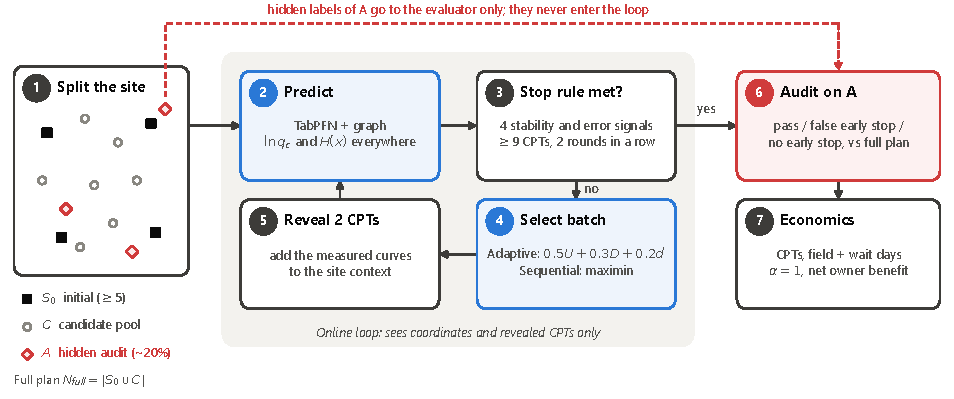
\includegraphics[width=\linewidth]{fig01_workflow.pdf}
\caption{Investigation loop. The hidden audit set $A$ is read only by a separate evaluator after the stop. All
policies share the initial set $S_0$, the candidate pool $C$ and $A$.}
\label{fig:workflow}
\end{figure}
